\section{연구 과정}

\subsection{하드웨어 제작}

\subsubsection{사용한 부품}

%%박기현샘 선정한 부품들의 특징은 무엇이며 왜 아래 부품들을 선정하였는지 추가할 것

천체망원경 모터 초점 조절 장치 컨트롤러를 제작하기 위해서 필요한 부품들을 선정하였다. 각각의 부품의 특징과 스펙을 아래에 정리하였다. 

\begin{description}[font=$\bullet$~\normalfont\scshape\color{red!50!black}]
	\item [ARDUINO NANO] 모터 초점 조절 장치 컨트롤러를 만드는 데 있어 가장 중요한 부품으로, 일종의 작은 컴퓨터와 같은 역할을 한다. Arduino는 마이크로 컨트롤러를 달고 있는 기판으로, Arduino의 여러 가지 핀에 전선을 연결한 뒤에 코딩하여 Arduino에 올리면 Arduino가 코딩된 내용을 그대로 실행할 수 있도록 하는 hardware이다. 내부에 컴퓨터 역할을 하는 MPU인 ATmega328가 탑재되어 있으며, 5V를 공급할 시에 작동한다. 크기는 45mm x 18mm이다.
	\item [0.96" oled screen I2C] Arduino와 I2C 방법으로 통신을 할 수 있는 OLED 스크린이다. 여러 가지 정보가 전달되며, 모터를 얼마나 돌릴 것인지, 혹은 얼마나 돌려져 있는지 등이 표현될 수 있다.
	\item [DHT22] 온도와 습도를 측정할 수 있는 감지기로, -40~80℃의 넓은 온도 측정범위와 약 0.5℃밖에 없는 오차를 가지고 있다. 이를 통해 온도나, 렌즈의 온도 상태를 볼 수 있으며, 이를 사용하면 좀 더 정밀한 측정이 가능할 것이다.
	\item [Apem MJTP1230B 버튼스위치] 누르는 버튼의 일종으로, 다리가 4개 달린 상태에서 같은 방향에 있는 2개의 전선이 연결된 방식의 버튼이다. 내부의 pull-up 저항을 활용하면 Arduino와 직접 연결하는 것으로 작동시킬 수 있다.
	\item [BP5277-90] 모터를 돌리기 위해서는 12V의 전압이 필요하다. 즉, 12V의 전압을 이용하여 모터를 돌리면서 Arduino를 실행시키기 위해서는 12V를 Arduino의 입력전압인 5V까지 낮출 필요가 있다. 이에 regulator와 축전기를 활용하여 가장 안전하게 5V까지 전압을 낮출 수 있는 regulator를 선택하였다.
	\item [HC-06 bluetooth] 무선통신 장치이다. 여러 가지 무선통신 장치 중에서 블루투스 module의 역할을 하고 있다.
	\item [LED 3mm 90', Ohmite OD473JE] 전원이 여러 개가 존재할 수 있으므로, 모터가 돌아갈 수 있는 전압인 12V의 외부전압이 들어왔을 때만 LED가 깜빡일 수 있게 하여 모터가 돌아갈 수 있는 전압이 되었는지 확인할 수 있도록 하는 역할을 하고 있다.
	\item [Panasonic EEA-GA1C100H] 모터를 돌리는 상황에서 큰 전류를 사용하기 때문에 전류가 역방향으로 흐르는 등의 문제를 방지하기 위하여 100μF의 축전기를 사용하였다.
	\item [SparkFun WRL-13678 (ESP8266, ESP01)] 무선통신 장치이다. 여러 가지 무선통신 장치 중에서 WIFI 모듈을 담당한다. 입력전압이 5V가 아닌 3.3V이다.
	\item [Sprague 1C10X7R104K050B] 부품별로 각각 연결된 축전기로, 모두 같은 전압 차를 가지고 있지만, 전류의 noise filtering을 하는 역할로, 필수적으로 사용되었다.
	\item [TMC2100 (DRV8825)] 스테핑 모터를 돌리는 데 있어서 전류를 쉽게 조절할 수 있게 해주는 module이다. 이뿐만이 아니라 모터를 좀 더 세밀하게 돌릴 수 있게 해주는(스텝 당 돌아가는 각도를 줄여주는) 마이크로 스텝을 구현 가능한데, DRV8825의 핀 중 M1, M2, M3의 up, down을 조절하여 full step을 원래 각도와 비교하면 얼마나 적게 돌릴 것인지 결정할 수 있게 한다. 본 모델은 최대 1/32까지의 마이크로 스텝이 가능하다.
	\item [TE Connectivity/AMP 5525258-3 및 Wurth Elektronik 694106301002] 12V 외부전원과 모터를 연결하는 선을 연결할 수 있게 하는 module이다.
\end{description}

\subsubsection{프로토 타입 회로 제작}

주어진 부품들을 하나하나 연결하여 만능기판에 와이어로 납땜을 하여 Figure \ref{fig:prototype}\과 같은 프로토 타입을 회로를 제작하였다. 

\begin{figure}[h]
	\begin{center}
		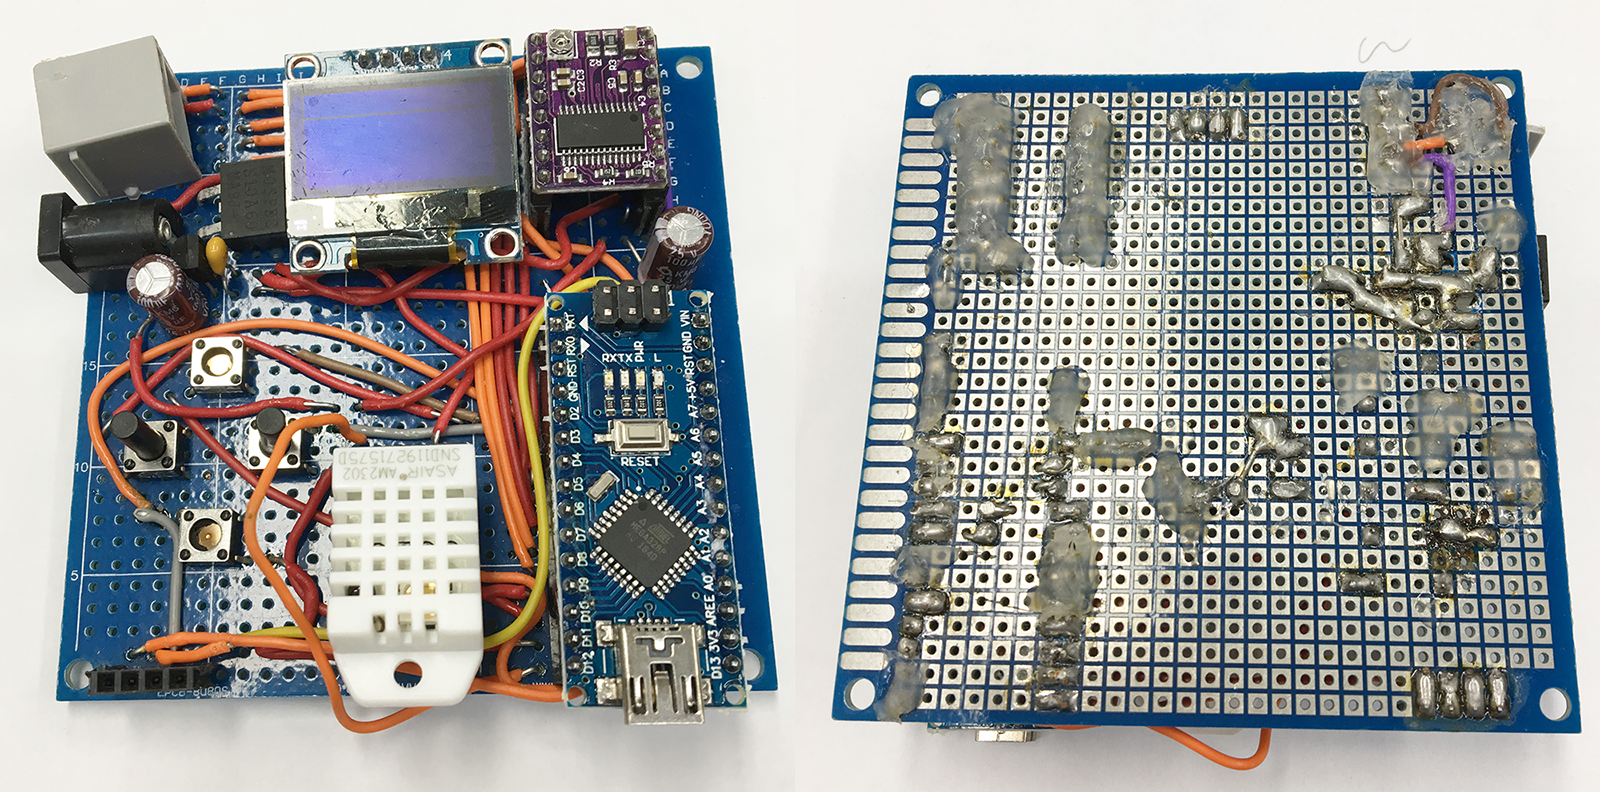
\includegraphics[width=0.9\linewidth]{prototype} 
		\caption{prototype}
		\label{fig:prototype}
	\end{center}
\end{figure}


\subsubsection{회로도 작성}


생각보다 Circuitmaker 프로그램의 사용법을 숙지하는 데 오랜 시간이 걸렸기 때문에, 그사이에 진행된 연구에서는 만능기판에 여러 가지 부품들을 전선으로 연결하여 사용하는 방법을 택하였고, 연구가 진행되어 만능기판이 복잡해짐에 따라서 여러 프로그램의 도움을 받게 되었다.\\

연구 초기과정에서는 Arduino와 직접 연동이 가능한 ‘Fritzing’이라는 프로그램을 사용하였지만, 연구가 진행될수록 다른 부품들과 실제로 구현이 가능한 PCB 회로기판을 만들 수 있어야 했기 때문에 보편화한 PCB 회로제작 프로그램이면서 ‘협업’ 기능을 이용하여 동시에 수정이 가능한 ‘Circuitmaker’라는 프로그램을 사용하게 되었다.

각 부품을 사용할 때에는 각 부품의 허용 전류와 같은 여러 가지 특징들을 생각하여 회로를 배선해야 한다. 예를 들어 WIFI 모듈인 ESP8266과 같은 경우 그 입력전압이 Arduino의 출력 전압인 5V가 아닌 3.3V이기 때문에 주의하여야 한다. 또한, 각 부품의 칩별로 제조한 회사의 data sheet를 참조하여 부품을 사용하면서 여러 가지 문제점들을 미리 방지하였다.\\
특히 5V를 3.3V로 바꾸는 과정에서는 전압 나눔 회로를 이용하여 전압을 나눌 수 있으나, 12V를 5V로 바꾸는 과정에서는 전류를 제어하는 것이 필요하므로 부득이하게 regulator를 사용하게 되었다.


Figure \ref{fig:Schematic_Prints}\는 최종 완성한 기판의 회로도이다.
\begin{figure}
	\begin{center}
	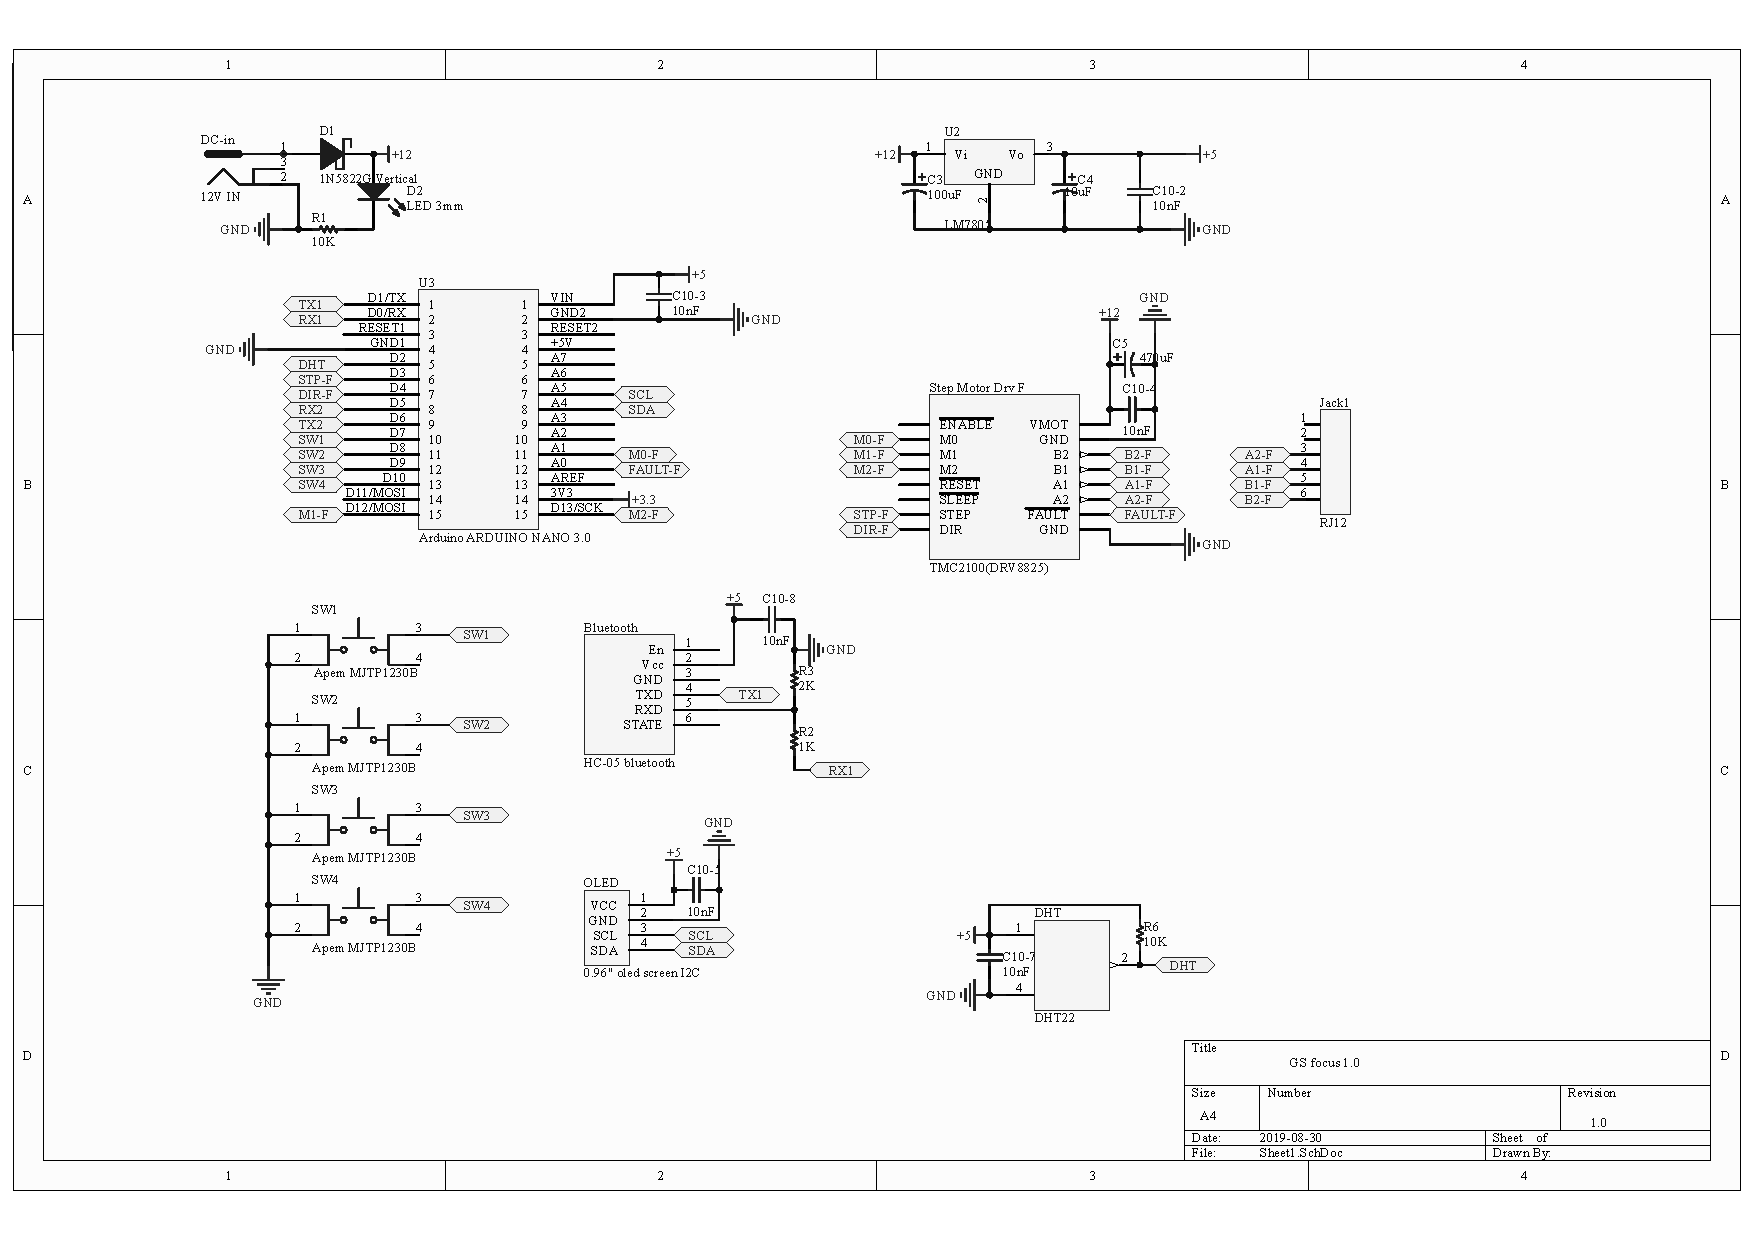
\includegraphics[width=1\linewidth]{Schematic_Prints_color}
	\caption{회로도}
	\label{fig:Schematic_Prints}
	\end{center}
\end{figure}


\subsubsection{기판 제작}
서킷 메이커 프로그램으로 회로를 그린 후 PCB를 디자인 하였다. 
%%박기현 샘  PCB를 디자인하기 위해 와이어링, 부품 배치, 폴리곤 푸어 등을 한 과정을 추가할 것
회로도에 따라 부품들이 와이어로 연결되어 있으므로 적절하게 배치하여 ......    PCB를 제작하였다. Figure \ref{fig:prototype}\은 서킷 메이커로 디자인한 PCB의 삼차원 모습을 나타낸다.

\begin{figure}[h]
	\begin{center}
	\begin{subfigure}{0.45\textwidth}
		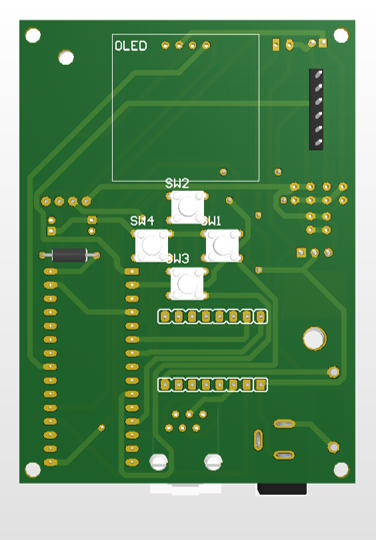
\includegraphics[width=0.9\linewidth]{pcbfront_3d} 
		\caption{Front}
		\label{fig:pcbfront_3d}
	\end{subfigure}
	\begin{subfigure}{0.45\textwidth}
		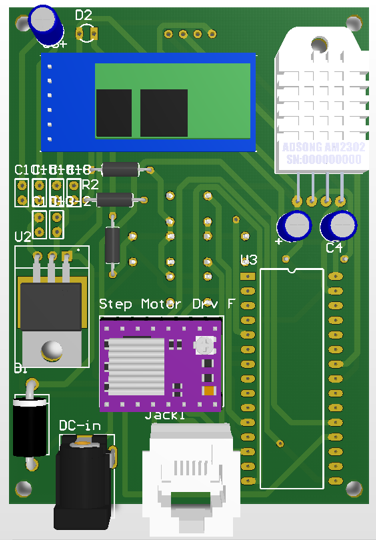
\includegraphics[width=0.9\linewidth]{pcbback_3d}
		\caption{Back}
		\label{fig:pcbback_3d}
	\end{subfigure}
	\caption{Circuit maker로 디자인한 PCB}
	\label{fig:pcb}
	\end{center}
\end{figure}

Figure \ref{fig:pcbcircuit}\은 처음 제작한 PCB Version 1 이다. PCB Version 1은 크기가 너무 크게 제작되었다.
\begin{figure}[h]
	\begin{center}
	\begin{figure}{0.9\textwidth}
		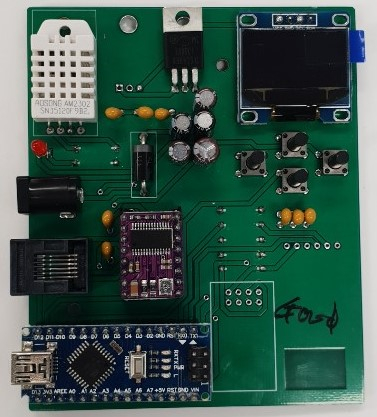
\includegraphics[width=0.9\linewidth]{pcbcircuit}
		\caption{PCB Ver. 1로 완성한 회로}
		\label{fig:pcbcircuit}
	\end{figure}
	\end{center}
\end{figure}

%%박기현 샘  이후 PCB는 어떤 점을 개선하였는지

\subsection{펌웨어 개발}

Arduino를 이용하여 모터 초점 조절 장치를 만드는 데 필요한 기술들은 크게 4가지이다. 먼저, Arduino와 모터 드라이버(DRV8825)를 이용하여 모터를 돌릴 수 있어야 한다. 두 번째로, 스위치를 활용하여 모터의 움직임을 조절할 수 있게 하였다. 세 번째로, 모터를 조절한 것을 노트북에 연결되지 않고 12V의 외부전원만 연결된 상황에서도 모터가 얼마나 돌아갔는지를 확인할 수 있도록 모터가 얼마나 돌아가 있는지, 혹은 이로 인해 늘어난 경통의 길이가 얼마나 되는지 확인할 수 있도록 Arduino를 이용하여 OLED 판을 실행시켜 진행 상황을 확인할 수 있게 하여야 한다. 마지막으로, 모터가 너무 많이 돌아간 경우나 새로운 모터에 모터 컨트롤러를 사용하는 경우 이를 복원시키기 위해 표시된 숫자를 초기화하는 과정이 필요하다.\\
펌웨어를 개발하는 과정에서 위의 4가지 기능들이 들어갈 수 있도록 하였으며, 추가로 모터의 step을 옮기는 과정에서 다른 모터 포커서 컨트롤러들의 장점을 융합하여 편리하게 사용할 수 있도록 하였다.\\
먼저, 메뉴 기능을 통해 자신이 원하는 기능을 직접 선택할 수 있도록 하였다. 이를 통하여 모터를 연속적으로 돌리는 기능과 미리 설정한 일정 값 정보를 돌릴 수 있도록 지원한다. 특히 연속적으로 돌리는 기능은 버튼을 오래 누를수록 더 빠르게 돌 수 있도록 하여 효율성을 높였다. 또한, 모터를 돌리는 것뿐만이 아니라 자신이 얼마나 돌렸는지 표시하는 기능을 포함하였다.


\subsection{ASCOM Protocol}

모터 초점 조절 장치를 활용하기 위해서는 별의 크기를 분석해서 돌려야 하므로 컴퓨터와의 연동을 위하여 초점 조절 장치의 ASCOM 드라이버를 C\# 코딩을 이용하여 제작한다. ASCOM 드라이버를 이용하면 카메라로부터 정보를 컴퓨터가 받아서 데이터를 분석하고, 이 분석한 데이터를 이용하여 모터를 어떻게 조절해야 할지 명령을 내리면 ASCOM 드라이버를 통해 정보를 전달하여 모터를 제어한 대로 조절이 가능하다.\\
현재 우리가 사용하는 프로그램은 ASCOM에서 만든 프로그램이고, ASCOM의 프로그램 대부분은 그 회사만의 표준 Protocol을 사용한다. 따라서 우리가 만드는 모터 초점 조절 장치 컨트롤러를 ASCOM Protocol에 따라 정보를 전달할 수 있도록 하면 일반 컴퓨터에 있는 ASCOM 프로그램을 이용하여 우리가 제작한 모터 초점 조절 장치 컨트롤러를 사용할 수 있도록 하는 것이 핵심이라고 할 수 있다.


\subsection{사용한 망원경}



